\documentclass[a4paper,10pt]{article}
\usepackage[margin=0.95in, top=1in,bottom=1.1in]{geometry}
\usepackage{amsmath}
\usepackage{gensymb}
\usepackage{graphicx}
\usepackage{mathtools}
\usepackage{booktabs}
\usepackage{multirow}
\usepackage{mathtools}
\usepackage{caption}
\usepackage{parskip}
\usepackage{tikz}
\usepackage{csquotes}
\usepackage{hyperref}
\usepackage{dsfont} % use expectation E
\renewcommand\rmdefault{ptm} % use Times
\let\boldtheta\theta % make theta into vector
\renewcommand{\theta}{\boldsymbol{\boldtheta}} % make theta into vector
\renewcommand{\d}{\: \mathrm{d}} % fix d in integrals
\usepackage{scrextend} % for lists
\newcommand{\x}{\mathbf{x}}

\title{\vspace*{-2.45em}\textbf{Project Proposal}\\ \vspace{0.25em} \Large Investigating Bayesian Inference in Continual Learning\vspace*{-0.9em}}

\author{M. E. Tong, supervised by S. Farquhar and Y. Gal}

\date{}

\begin{document}

\maketitle

%Background: the theory or application areas;
%General open questions;
%Selection of particular question for study;
%Proposed method;
%Draft Timetable;
%Signature of Project Supervisor.

\vspace{-1.5em}
For real-world problems, it is vital that intelligent agents have the capacity to learn and remember a variety of tasks \cite{ewc}. Continual learning refers to online multi-task learning where tasks are learned sequentially, with datasets discarded after training. It is of particular importance for applications for which retaining old datasets is unethical, undesireable, illegal or imprudent, such as for private data relating to individuals \cite{unifying, robust}.
%Maybe give some concrete examples where this might be useful? E.g., private data that must be deleted every 6m, or adapting a robot to work on multiple terrains after deployment.

The major problem in the field is that of catastrophic forgetting. New learning often causes neural networks to rapidly forget old learning \cite{catastrophic}. The challenge is to balance learning new tasks whilst remembering previous ones. Though promising results have been published in the field of continual learning, clear shortcomings have been identified in many of the current approaches and evaluations, such as a dependency on re-training on previous datasets or tasks \cite{robust}. 

The most recent advances in continual learning have favoured a prior-focused approach, such as variational continual learning \cite{vcl}, elastic weight consolidation \cite{ewc}, synaptic intelligence \cite{si}, Riemannian walk \cite{rw} and Kronecker factored online Laplace approximation \cite{ritter}. These prior-focused approaches use the posterior or other parameters from previous tasks as priors for new tasks. Likelihood-based approaches, such as Deep Generative Replay \cite{dgr}, are based on pseudo-rehearsal \cite{robins}, simulating previous datasets in order to estimate their log-likelihood according to the new model. There have also been approaches based on dynamic architectures. %Rusu 2016, Li and Hoiem 2017

%This section seems basically good. In general, a useful way to frame an introduction is to simply state the context, the problem, your solution, and your specific contributions. Here, of course, your prompt is a bit different. For the final report, let's work on getting this language more succinct and less flowery. For now it's probably fine.

\vspace{-1.25em}
\subsubsection*{Variational Continual Learning}

\vspace{-1em}
Further investigation into the variational continual learning (VCL) approach \cite{vcl} is warranted. At the moment, VCL's good performance is dependent on re-training on small coresets retained from previous datasets \\\cite{robust}, but improvements to the approach may eliminate the need for these coresets, which cannot be assumed to be available for all continual learning applications. %which would better reflect true continual learning. %Coresets cannot always be used, not available for many applications % Aesthetic reasons aside - why is this useful? 

VCL demonstrates a prior-focused Bayesian approach to continual learning, where the posterior for the previous tasks is used as the prior when training on the new task dataset. This is a correct and intuitive way of allowing the previous tasks to strongly influence prediction, whilst allowing the parameters to adapt to the new task.%Is it intuitive? Or is it just correct? If we were unconstrained by compute - the Bayesian approach would be optimal (given selection of appropriate prior). 

\vspace{-1.85em}
\begin{equation}\label{eq:1}
\begin{split}
\underbrace{p(\theta | \mathcal{D}_{1:t})}_{\mathclap{\text{new posterior}}} \propto \underbrace{p(\theta | \mathcal{D}_{1:t-1})}_{\substack{\text{previous posterior}\\ (\text{new prior})}} \underbrace{p(\mathcal{D}_t | \theta)}_{\text{likelihood}}
\end{split}
\end{equation}

\vspace{-0.95em}
However, the true posterior $p(\theta | \mathcal{D}_{1:t})$ is computationally intractable, so we must approximate it. Improvements to this approximation must be key to performance, since this approach is optimal with exact Bayesian inference. % More - we know the full Bayesian inference is optimal. But this isn't working. So which approximation is the one that breaks it?

% I think normally we'd frame this as being performed using mean-field variational inference. MFVI minimizes the evidence lower bound (ELBO) loss. That ELBO loss is expressed using a KL divergence between the posterior and variational distribution.
The posterior approximation in VCL employs mean-field variational inference (VI). Variational inference aims to minimise the Kullback-Leibler (KL) divergence over a model family of possible posteriors $\mathcal{Q}$ in order to yield a tractable normalised approximation $q_t(\theta)$ to the true posterior $p(\theta | \mathcal{D}_{1:t})$. We define $q_0(\theta)$ to be the prior, $p(\theta)$.

\vspace{-2.em}
\begin{equation}\label{eq:3}
\begin{split}
\underbrace{p(\theta | \mathcal{D}_{1:t})}_{\mathclap{\substack{\text{new true}\\ \text{posterior}}}}\approx \underbrace{q_t(\theta)}_{\mathclap{\substack{\text{new posterior}\\ \text{approximation}}}} &=\underset{q\in\mathcal{Q}}{\mathrm{arg}\mathrm{min}} \: \mathrm{KL}\Big(q(\theta)\:||\:\frac{1}{Z_t}\underbrace{q_{t-1}(\theta)}_{\mathclap{\substack{\text{previous posterior} \\ \text{approximation}}}}\overbrace{p(\mathcal{D}_t|\theta)}^{\mathclap{\text{likelihood}}} \Big)\\
\end{split}
\end{equation}

\vspace{-0.6em}
In VI, this minimisation is typically done via a maximisation of the variational evidence lower bound (ELBO). 

\vspace{-1.9em}
\begin{equation}\label{eq:4}
\begin{split}
\mathrm{ELBO}= \underbrace{{\textstyle\sum}_{n=1}^{N_t} \> \mathds{E}_{\theta \sim q_t(\theta)}\big[\log p(y_t^{(n)} \:| \:\theta, \x_t^{(n)})\big]}_{\substack{\text{expected log-likelihood}\\\text{of new model over the new data}}} \> -  \> \underbrace{\mathrm{KL}\big(q_t(\theta)\:||\:q_{t-1}(\theta)\big)}_{\mathclap{\substack{\text{difference between new model and}\\\text{previous posterior approximation}}}}
\end{split}
\end{equation} %{\textstyle\sum}
%Here, $\theta$ are the parameters, $\mathcal{D}_i$ is the $i$\textsuperscript{th} dataset, $q_i(\theta)$ is the posterior approximation following the $i$\textsuperscript{th} dataset, $Z_t$ is the intractable normalisation constant which is irrelevant for minimisation.

\vspace{-0.8em}
Crucially, this is exact Bayesian inference, $q_t(\theta)=p(\theta | \mathcal{D}_{1:t}) \>\, \forall t$, if two criteria are met at every step:

\begin{enumerate}
\item The true posterior is a member of the model family $\mathcal{Q}$.
\vspace{-0.2em}
\item The optimisation achieves the maximum model evidence.
% Optimisation is a big problem, as we aren't sure that we find the minimum
% We make a big assumption that we are actually getting a minimum KL divergence

%I'd emphasise that in MFVI we only optimize a bound on this KL divergence.
\end{enumerate}

Since the posterior approximation occurs after every task is learned, improving this approximation is important to prevent error propagation across different tasks. We therefore suggest that investigation into improvements to these two criteria should be the aims of the project.

\vspace{-1em}
\subsubsection*{Aims of the project}

\vspace{-1em}
%You often say "we suggest" or "we suspect". This makes sense if we aren't confident about things. But hopefully we can remove this sort of language mostly, and replace it with clear statements of what we do know. In this case, we know that the full-covariance version has been implemented in the past (outside a CL setting) and that we can test this easily using existing code. MCMC will just be a bit more complex to implement and doesn't match the baselines as well.
An investigation into an improvement to the first criterion is the most promising, as it is likely that the model family used in VCL is not sufficient to approximate the posterior well. The primary aim of the project is therefore to see if using a more adaptable model family results in better performance:
% So we're pretty confident it doesn't lie in this model family
% Relaxation

\begin{enumerate}
\item \textbf{Using full covariance Gaussian distributions for the model family $\mathcal{Q}$.}

VCL uses a Gaussian mean-field approximate posterior, with diagonal covariance: %sigma^2_{t,d}
\[q_t(\theta) = \prod^D_{d=1} \mathcal{N}(\boldtheta_{t,d}; \mu_{t,d}, \sigma^2_{t,d})\]
% correlation elements, non-diagonal elements
We expect that a full covariance Gaussian distribution will be able to approximate the posterior more accurately by including off-diagonal correlation elements in the covariance matrix, which can be significant. Simple diagonal covariance Gaussian distributions approximate the posterior too conservatively, placing no probability mass where the posterior is small \cite{mackay1995}. The minimum KL fit obtained with the full covariance model family should therefore be better than that obtained with the diagonal covariance model family. %MacKay 1992 thinks off-diagonal elements are significant.

\begin{center}
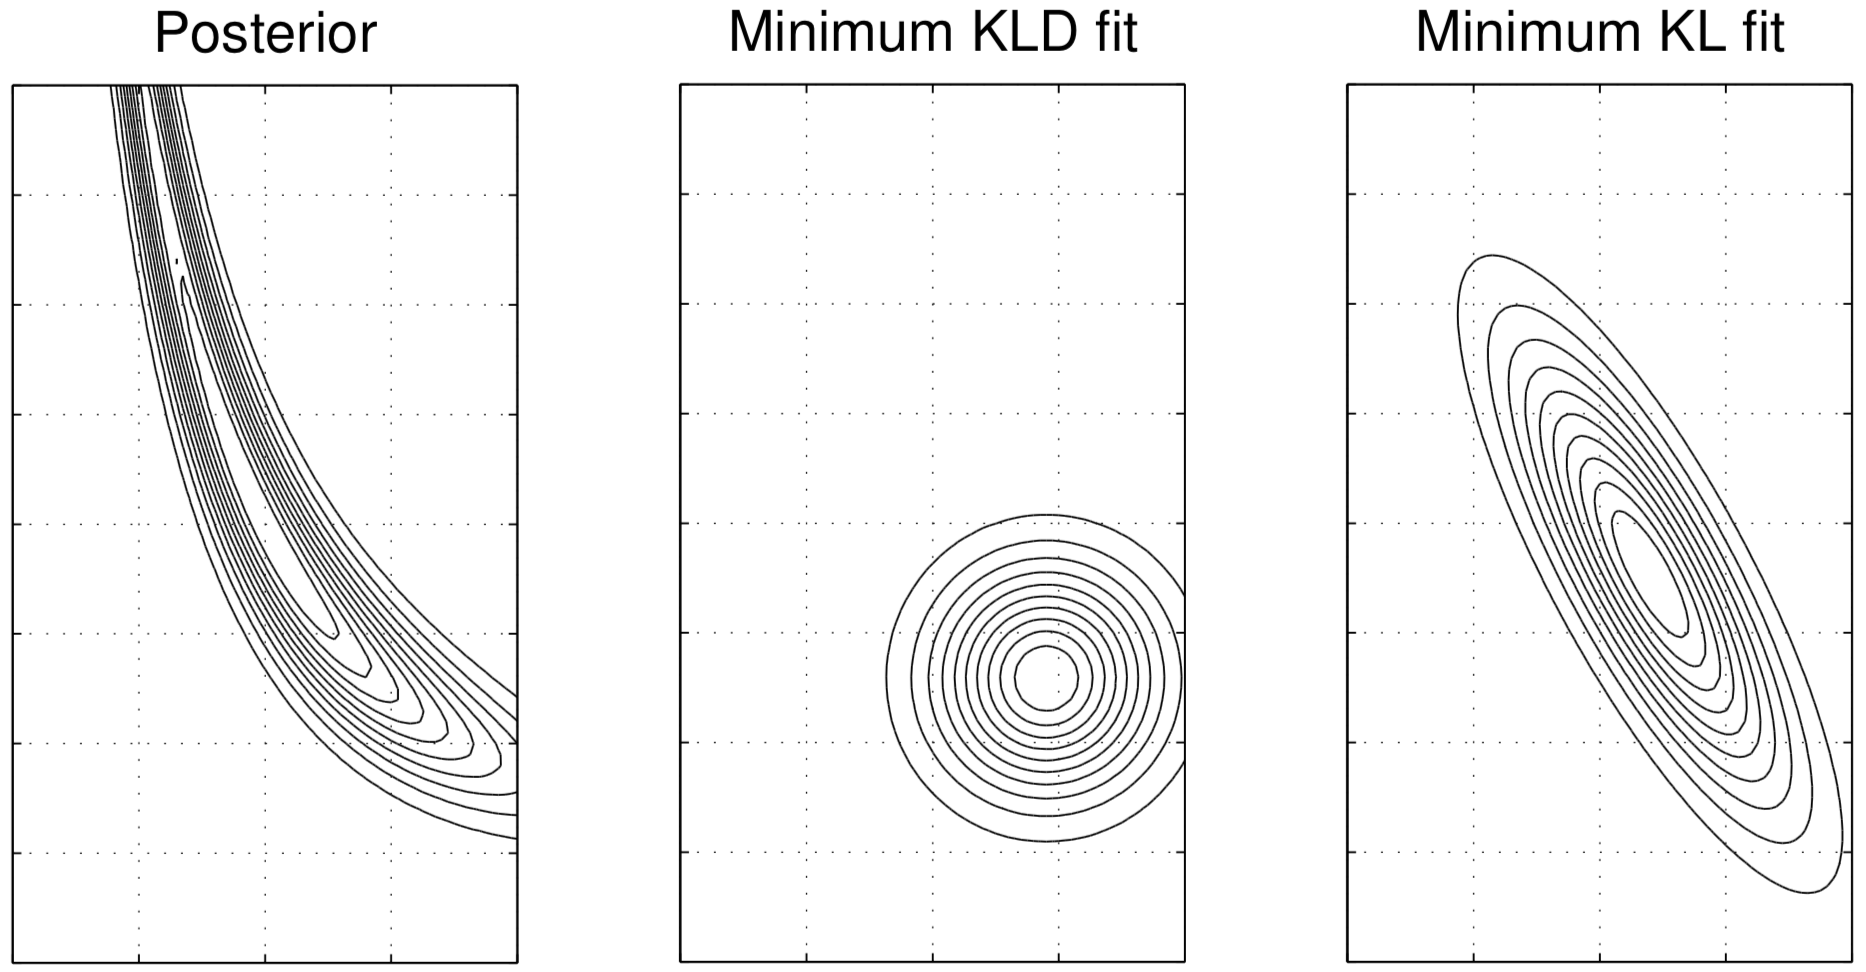
\includegraphics[width=0.7\textwidth]{approximations}
 \label{figure:family}
\end{center}
{Figure 1: Comparison of posterior distribution approximations on a synthetic example with two parameters. A full covariance Gaussian distribution (KL) results in a much improved approximation to the posterior than the diagonal covariance Gaussian distribution (KLD), with a lower residual KL value and better KL fit. `More flexible distributions \textelp{} simply give better approximations to the true posterior'.
\cite{bishopbarber}}
%A diagonal covariance Gaussian distribution (KLD) results in KL\textsubscript{res} = 4.6, whereas a full covariance Gaussian distribution (KL) results in an improved KL\textsubscript{res} = 3.9. \cite{bishopbarber}}.

A tractable algorithm for posterior approximation with a full covariance Gaussian distribution has been demonstrated \cite{bishopbarber}. %Elaborate?

\end{enumerate}
\vspace{0.5em}
An investigation into an improvement to the second criterion may also be promising. Approximate Bayesian inference is typically carried out with either VI or Markov Chain Monte Carlo (MCMC). The secondary aim of the project is therefore to see if using MCMC results in better performance:
\begin{enumerate}
\setcounter{enumi}{1}
\item \textbf{Using a Markov Chain Monte Carlo method for posterior approximation.}

Using a Monte Carlo method to sample from the posterior distribution gets close to exact Bayesian inference in practice, and is advantageous in that it does not impose as many assumptions about the shape of the posterior distribution \cite{hinton}.
% Not quite - interestingly. There was a recent paper by Titsias that uses Gaussian Processes for CL that would be worth reading.

We expect that Hamiltonian Monte Carlo (HMC) is a promising MCMC method to use for approximate inference. HMC is a principled Hamiltonian dynamics-based MCMC method which has been applied successfully to Bayesian neural networks \cite{neal1995}. It systematically and coherently traverses the state space, avoiding the slow exploration typical of random walk proposals \cite{neal2012}. This is particularly useful in high-dimensional spaces, where we must use information about the space geometry for an efficient exploration. Gradient-based algorithms such as HMC tend to be more robust and geometrically ergodic over a larger class of target distributions than non-gradient based algorithms, yielding `stronger guarantees on the validity of the resulting estimators' \cite{betancourt}.
% second-gradient - calculating Hamiltonian is really expensive for high dimensional spaces
% HMC sets cap on size of neural network we can use
\end{enumerate}


\subsection*{Approximate Timeline}

\begin{tabular}{l|l}
\hline
March 	& Review literature\\
April	& Review literature; write project proposal\\
May		& Review literature; use non-continual BNN to compare diagonal and full model families\\ % You may also need more literature review time. Especially important to be familiar with Barber and Bishop.
June 	& Begin continual learning comparison implementation\\
July	& Continue with continual learning comparison and begin MCMC implementation \\
August	& Continue with MCMC implementation; finish writing up results\\% I would set aside some time for understanding the results and interpreting/writing up
September 2 & Hand-in date\\
\hline
\end{tabular}

%\subsection*{Project supervisors' signatures}

%\begin{labeling}{projectsupervisors}
%\vspace*{2.25em}
%\item[S. Farquhar] \rule{5cm}{1pt}
%\vspace*{2.5em}
%\item[Y. Gal] \rule{5cm}{1pt}
%\end{labeling}



\begin{thebibliography}{8}

\bibitem[Barber \& Bishop, 1998]{bishopbarber} D. Barber, C. M. Bishop, 1998. \textit{Ensemble Learning in Bayesian Neural Networks}. Neural Networks and Machine Learning, Springer, 215-237. \href{https://www.microsoft.com/en-us/research/wp-content/uploads/2016/02/bishop-ensemble-nato-98.pdf}{Link to paper}

\bibitem[Betancourt, 2017]{betancourt} M. Betancourt, 2017. \textit{A Conceptual Introduction to Hamiltonian Monte Carlo}. \href{https://arxiv.org/abs/1701.02434}{arXiv:1701.02434v2}

\bibitem[Chaudhry et al., 2018]{rw} A. Chaudhry, P. K. Dokania, T. Ajanthan, P. H. S. Torr, 2018. \textit{Riemannian Walk for Incremental Learning: Understanding Forgetting and Intransigence}. \href{https://arxiv.org/abs/1801.10112}{arXiv:1801.10112v3}

\bibitem[Farquhar \& Gal, 2019]{unifying} S. Farquhar, Y. Gal, 2019. \textit{A Unifying Bayesian View of Continual Learning}. \href{https://arxiv.org/abs/1902.06494}{arXiv:1902.06494v1}

\bibitem[Farquhar \& Gal, 2018]{robust} S. Farquhar, Y. Gal, 2018. \textit{Towards Robust Evaluations of Continual Learning}. \href{https://arxiv.org/abs/1805.09733}{arXiv:1805.09733v2}

\bibitem[Hinton \& van Camp, 1993]{hinton} G. E. Hinton, D. van Camp, 1993. \textit{Keeping the
Neural Networks Simple by Minimizing Description Length of the Weights}. \href{http://www.cs.toronto.edu/~fritz/absps/colt93.pdf}{Link to paper}

\bibitem[Kirkpatrick et al., 2017]{ewc} J. Kirkpatrick, R. Pascanua, N. Rabinowitza, J. Venessa, G. Desjardinsa, A. A. Rusua, K. Milana, J. Quana, T. Ramalhoa, A. Grabska-Barwinskaa, D. Hassabisa, C. Clopathb, D. Kumarana, and R. Hadsella, 2017. \textit{Overcoming catastrophic forgetting in neural networks}. \href{https://arxiv.org/abs/1612.00796}{arXiv:1612.00796v2}

%\bibitem[MacKay, 1992]{mackay1992} D. J. C. MacKay, 1992. \textit{A Practical Bayesian Framework for Backpropagation Newtorks}. \href{https://authors.library.caltech.edu/13793/1/MACnc92b.pdf}{Link to paper}

\bibitem[MacKay, 1995]{mackay1995} D. J. C. MacKay, 1995. \textit{Probable networks and plausible predictions - a review of practical Bayesian methods for supervised neural networks}. \href{https://citeseerx.ist.psu.edu/viewdoc/download;jsessionid=F4F7C99DECF23AEDF5BAAF5E25DE86F9?doi=10.1.1.136.4011&rep=rep1&type=pdf}{Link to paper}

\bibitem[McCloskey \& Cohen, 1989]{catastrophic} M. McCloskey, N. J. Cohen, 1989. \textit{Catastrophic Interference in Connectionist Networks: The Sequential Learning Problem}. Psychology of Learning and Motivation, Volume 24, 109-165.

\bibitem[Neal, 2012]{neal2012} R. M. Neal, 2012. \textit{MCMC using Hamiltonian dynamics}. \href{https://arxiv.org/abs/1206.1901}{arXiv:1206.1901v1}

\bibitem[Neal, 1995]{neal1995} R. M. Neal, 1995. \textit{Bayesian Learning for Neural Networks}. \href{http://citeseerx.ist.psu.edu/viewdoc/download?doi=10.1.1.446.9306&rep=rep1&type=pdf}{Link to paper}

\bibitem[Nguyen et al., 2017]{vcl} C. V. Nguyen, Y. Li, T. D. Bui, R. E. Turner, 2017. \textit{Variational Continual Learning}. \href{https://arxiv.org/abs/1710.10628}{arXiv:1710.10628v3}

%\bibitem[Ratcliff, 1990]{connectionist} R. Ratcliff, 1990. \texdtit{Connectionist Models of Recognition Memory: Constraints Imposed by Learning and Forgetting Functions}. Psychological Review, Vol.97, No. 2, 285-308.

\bibitem[Ritter et al., 2018]{ritter} H. Ritter, A. Botev, D. Barber, 2018. \textit{Online Structured Laplace Approximations For Overcoming Catastrophic Forgetting}. \href{https://arxiv.org/abs/1805.07810}{arXiv:1805.07810v1}

\bibitem[Robins, 1995]{robins} A. Robins. \textit{Catastrophic forgetting, rehearsal, and pseudorehearsal}. Connection Science: Journal of Neural Computing, Artificial Intelligence and Cognitive Research, Volume 7, 123-146.

\bibitem[Shin et al., 2017]{dgr} H. Shin, J. K. Lee, J. Kim, J. Kim, 2017. \textit{Continual Learning with Deep Generative Replay}. \href{https://arxiv.org/abs/1705.08690}{arXiv:1705.08690v3}

\bibitem[Zenke et al., 2017]{si} F. Zenke, B. Poole, S. Ganguli, 2017. \textit{Continual Learning Through Synaptic Intelligence}. \href{https://arxiv.org/abs/1703.04200}{arXiv:1703.04200v3}
%\bibitem[Liu \& Chen, 1998] J. S. Liu, R. Chen, 1998. \textit{Sequential Monte Carlo Methods for Dynamic Systems}. Journal of the American Statistical Association, Vol. 93, No. 443, pp. 1032-1044.




\end{thebibliography}



\end{document}
